\documentclass[german,version-2022-01]{uzl-thesis}


% Copy this file as a template for your thesis. You will have to take
% action at all places marked by
%
% !!!!!!!!!!!!!!!!!!!!!!!!!!!!!!!!!!
% !!! Your action is needed here !!!
% !!!!!!!!!!!!!!!!!!!!!!!!!!!!!!!!!!
%
% The first place your action is needed is the first line of this
% document:
%
%
% Language of the thesis:
%
% You must use either 'german' or 'english' above, depending on the
% language used in the main text. This will automatically setup a lot
% of things in the background.
%
%
% Version of the class:
%
% You must specify which version of the thesis class is to be
% used. This is important in case the class style changes in later
% years, but we still want an older thesis to look the same, even when
% things are changed in the class.
%
% Do not change or remove the version-xxxx key.
%
%
% Text encoding:
%
% Your thesis *must* be encoded in utf8 (unicode), which is the
% default in most editors these days. Do *not* change this to latin8.



%%%
%
% Main setup:
%
%%%
%
% You must use the \UzLThesisSetup command to specify numerous things
% about your thesis. This includes the entries on the title page, the 
% abstracts, and the bibliography style. You do so by specifying
% so-called "values" for so-called "keys". For instance, 
% for the key "Autor" you must provide your name as the value. You do
% so by writing 'Autor = {Max Mustermann}', that is, the value is put
% into curly braces. You can use the \UzLThesisSetup command
% repeatedly and the order in which you provide the keys is not
% important. 
%
% Everything shown on the title page must be in German -- even
% if the thesis is written in English! Just insert German text for
% German keys and English text for English keys (like 'Abstract' needs
% English text, while 'Zusammenfassung' needs German text).

\UzLThesisSetup{
  %
  % !!!!!!!!!!!!!!!!!!!!!!!!!!!!!!!!!!
  % !!! Your action is needed here !!!
  % !!!!!!!!!!!!!!!!!!!!!!!!!!!!!!!!!!
  %
  % First, specify the institut or clinic at which the thesis was
  % written. You get the logo file from them (make sure it has the
  % correct size, namely the same as the example). If they do not have
  % a logo, the university's default logo is used.
  %
  % The 'verfasst' gets two arguments. Change the first to {an der}
  % for clinics, as in 'Verfasst = {an der}{Medizinischen Klinik I}'
  %
  Logo-Dateiname        = {uzl-thesis-logo-uzl.pdf},
  Verfasst              = {am}{Institut f\"ur Neuro- und Bioinformatik},
  %
  % The titles:
  %
  Titel auf Deutsch     = {
    Analyse einer DNA-Datenbank auf Mutationsstabilit\"at basierend auf (bio-)chemisch relevanter Molek\"uleigenschaften
  }, 
  Titel auf Englisch    = {
    Analysis of a DNA Database for Mutation Stability Based on (Bio-)Chemically Relevant Molecular Properties 
  },
  %
  % Author and supervisor:
  % 
  % Note that the 'Betreuer' or 'Betreuerin' is the supervisor, that
  % is, the professor who officially supervises the thesis. If there
  % is also an assistent of the professor who helped (typically a
  % lot), use 'Mit Unterstützung von' to thank that person. If the
  % thesis was mainly written 'externally' at some company or another
  % institute, point this out using 'Weitere Unterstützung'. 
  % 
  % For your own name, do *not* add things like "BSc" or "BSc
  % cand.". For the supervisor, you should normally include
  % "Prof. Dr." or "PD Dr." (ask your supervisor, what is
  % appropriate), but nothing more (so no
  % "Univ.-Prof. Dr. Dr. h.c. mult." unless your supervisor insists).  
  %
  Autor                 = {Leonie Nie\ss{}},
  Betreuerin            = {PD Dr. Amir Madany Mamlouk},
  % 
  % Optional: Supporting persons and institutions. The text should be
  % in German, even for an English thesis.
  %
  Mit Unterstützung von = {BSc. Nina Eichler},
  % 
  %   Weitere Unterstützung = {
  %     Die Arbeit ist im Rahmen einer Tätigkeit bei der Firma Muster GmbH
  %     entstanden.
  %   },
  %
  %
  % Your Degree Programm (Studiengang)
  %
  % Specify 'Bachelorarbeit' or 'Masterarbeit' and the degree
  % programme. Make sure the name of programme is correct and not
  % some abbreviation or some incorrect variant. For instance:
  % 'Medizinische Ingenierwissenschaft', but not 'MIW';
  % 'Medizinische Informatik', but not 'Medizin-Informatik';
  % 'Informatik', but not 'Informatik (SSE)'.
  %
  % Use German names for German programmes and English names for
  % English ones, so 'Infection Biology', not 'Infektionsbiologie'. 
  % For programmes that have a German bachelor and an English master,
  % use the German name for a bachelor thesis and the English name for
  % the master thesis.
  %
  Bachelorarbeit,
  Studiengang           = {Medizinische Informatik},
  %
  % Date on which the thesis is turned in German, formatted the
  % traditional German way:
  %
  Datum                 = \today,
  %
  % The English abstract. You must always provide abstracts in German
  % and in English. 
  %
  Abstract              = {
  
  },
  Zusammenfassung       = {
  
  },
  %
  % Optional: 'Danksagungen' (German) or 'Acknowledgements'
  % (English). Both keys are optional and both have the same effect of
  % adding an acknowledgements text after the abstracts and before the
  % table of contents.
  %
  %Acknowledgements      = {
  %  This is the place where you can thank people and institutions, do not try to do this on the title page. The only exception is in case you wrote your thesis while working or staying at a company or abroad. Then you should use the \Latex{Weitere Unterstützung} key to provide a text (in German) that acknowledges the company or foreign institute. For instance, you could use texts like »Die Arbeit ist im Rahmen einer Tätigkeit bei der Firma Muster GmbH entstanden« or »Die Arbeit ist im Rahmen eines Forschungsaufenthalts beim Institut für Dieses und Jenes an der Universität Entenhausen entstanden«. Do not name and thank individual persons from the company or foreign institute on the title page, do that here. 
  %},
  % Bibliography style: Choose between
  % 
  % 'Alphabetische Bibliographie'
  % for all degree programmes in the natural sciences 
  % 
  % 'Numerische Bibliographie'
  % alternative for all other degree programmes
  % 
  % Either will load biblatex and setup the citation methods and the
  % bibliography styles correctly. You should not mess with them.
  % 
  % Alphabetische Bibliographie,
  % Alternatively:
  Numerische Bibliographie
}




%%%%%%%%%%%%%%%%%%%%
%
% Styling the thesis
%
%%%%%%%%%%%%%%%%%%%%
%
% Creating a visually pleasing layout and choosing fonts is not
% easy. Furthermore, different people have different preferences. Of
% course, for the University of Lübeck, the dean of studies could just
% force everyone to use one specific layout and font, but that seems a
% bit drastic and, also, it seems nice that thesis by different people
% have an individual style even though they all stick to the same
% overall structure.
%
% For these reasons, I (Till Tantau) have spend quite some time on
% designing a flexible layout and styling mechanism for theses.
%
% Basically, the overall structure of the thesis is fixed by the
% thesis class and so are many structural elements. For instance, you
% cannot change the order in which the abstract and table of contents
% are shown, you cannot move the bibliography elsewhere, indeed, the
% bibliography style is also fixed. Likewise, the text on the title
% page is fixed.
%
% Although many things are fixed, you *can* change several other
% things. For instance, you can change the font used for the main
% text, you can change which font is used for titles and headings or
% you can change whether titles and headlines are centered or flushed
% left.
%
% There are many LaTeX packages for changing such things. You are
% kindly asked *not to use them*. Rather, use (only) the options
% offered by the thesis class. All possible choices and combinations
% there have been tested by me and produce nice results; what happens
% with other packages no one knows and might no longer conform to what
% is expected by the university. As you will see, you still have a
% lot of options.
%
%
% Technical note: All styling is done via the command
%
% \UzLStyle{...}
%
% where ... is a key-value list just as for \UzLThesisSetup. The
% difference is just that everything having to do with styling as
% controlled by \UzLStyle, while the more “formal” setup keys are
% controlled by \UzLThesisSetup.
%
%%%
%
% Designs
%
%
% A \emph{design} is a whole set of font and layout options bundled
% together. They have been chosen in such a way that a visually
% pleasing “overall appearance” results.
%
%
% \UzLStyle{computer modern oldschool design}
%
% The look of this design mimics the “classical” way a paper or report
% created with \LaTeX\ looks like: The Computer Modern font is used,
% bold face fonts are used for headlines, only black and white are
% used as colors. This design reminds me of older scientific
% documents, especially from the computer science community where
% \LaTeX\ was used very early.
%
%
% \UzLStyle{computer modern basic design}
%
% A slightly less “oldschool” version of the previous design. It is
% still a classic design in the sense that it uses the Computer Modern
% font and that it still has this “good old \LaTeX” look, but some
% more modern aspects (like colors!) have been added.
%
% Note that this design uses Myriad for the title page (one of the
% “modern aspect”), which means that his font must be installed.
%
%
% \UzLStyle{computer modern scholary design}
%
% In my opinion, this is the ultimate “scholary design”: The thesis
% will look like it has been typeset by hand some 150 years ago and
% then printed by a university press. There is really nothing “modern”
% about it and the word in the name of the design is just part of the
% name of the “Computer Modern” font.
%
%
% \UzLStyle{pagella basic design}
%
% A, well, basic design that uses the Pagella font rather than the
% Computer Modern font. Especially the bold face version of this font
% looks nicer than the Computer Modern counterpart. Also, Pagella,
% while still having a “bookish” look, still feels a bit fresher than
% Computer Modern. 
%
%
% \UzLStyle{pagella centered design}
%
% A variant of the basic Pagella design that centers all
% headlines. A nice alternative to the basic version.
%
%
% \UzLStyle{pagella contrast design}
%
% This design tries to create some visual friction by contrasting the
% sans serif headline font (in bold!) with the main text. I find it a
% visually very interesting combination.
%
%
% \UzLStyle{alegrya basic design}
%
% The third variant of the basic design, this time using the Alegrya
% font. 
%
%
% \UzLStyle{alegrya scholary design}
%
% The Alegrya version of the previous “scholary” design. Unlike the
% Computer Modern version, this design does not look old, but more
% fresh -- while still creating the impression that the text must be
% about a very scientific subject. 
%
%
% \UzLStyle{alegrya stylish design}
%
% The design is quite similar to the scholary version for the Alegrya
% font, but with even more modern additions. “Stylish” is the word
% that comes to my mind.
%
%
\UzLStyle{alegrya modern design}
%
% A design that uses the sans serif version of the Alegrya font for
% the headlines. This is a nice modern overall design.
%
%%%




%%%%%%%%
%
% Now, include the package you need here using \usepackage. 
%
% However, many standard packages are already loaded by the class:
%
% amsmath, amssymb, amsthm, babel, biblatex, csquotes, etoolbox,
% filecontents, fontspec, geometry, hyperref, tikz (with libraries
% arrows.meta, positioning and shapes), varioref, url 
%
% Indeed, in many cases you will not need any extra packages.
%
%%%%%%%





\begin{document}

%
% The title page and table of contents will be inserted automatically
% here. 
%


\chapter{Einleitung}
% In a German thesis write: \chapter{Einleitung}


% !!!!!!!!!!!!!!!!!!!!!!!!!!!!!!!!!!
% !!! Your action is needed here !!!
% !!!!!!!!!!!!!!!!!!!!!!!!!!!!!!!!!!
%
% Replace with your own introduction:
Fragestellung: Sind transmembrane Bereiche eines Proteins besonders Mutationsstabil \"uber polar requirements? Bzw. herrscht dort ein gro\ss{}er Konservierungsdruck, sodass sich die polar requirements in diesen Bereichen st\"arker konservieren und es somit nur wenig \"Anderung geben darf? 

Proteine sind biomolekulare Strukturen, die aus langen Ketten von Aminos\"auren bestehen. Diese Aminos\"auren sind durch Peptidbindungen miteinander verkn\"upft und bilden die prim\"are Struktur des Proteins. Die spezifische Sequenz der Aminos\"auren bestimmt die Faltung und damit die sekund\"are, terti\"are und quart\"are Struktur des Proteins, die f\"ur seine Funktion entscheidend ist. Proteine erf\"ullen eine Vielzahl von biologischen Funktionen, darunter Enzymaktivit\"at, Transport von Molek\"ulen, Immunabwehr und strukturelle Unterst\"utzung in Zellen und Geweben. Sie sind auch an Signaltransduktion und Zellkommunikation beteiligt. Transmembranproteine stellen eine spezielle Klasse von Proteinen dar, die in die Zellmembran eingelagert sind und sowohl die innere als auch die \"au\ss{}ere Zellumgebung beeinflussen. Diese Proteine besitzen oft hydrophobe Bereiche, die durch die Lipid-Doppelschicht der Zellmembran hindurchragen, sowie hydrophile Bereiche, die mit dem Zytoplasma oder der extrazellul\"aren Umgebung interagieren. Die Stabilit\"at von Transmembranbereichen ist entscheidend f\"ur die Funktion dieser Proteine. Mutationen in diesen Bereichen k\"onnen die Stabilit\"at und Funktion der Proteine beeintr\"achtigen, was zu verschiedenen Krankheiten f\"uhren kann. Daher ist das Verst\"andnis der Mutationsstabilit\"at in Transmembranproteinen von gro\ss{}er Bedeutung f\"ur die biomedizinische Forschung.

Dengue-Viren sind Arboviren, die haupts\"achlich durch Stechm\"ucken, insbesondere die Asiatische Tigerm\"ucke (Aedes albopictus), auf den Menschen \"ubertragen werden \cite{cramer_dengue-virus_2014}. Sie geh\"oren zu einer Gruppe von Erregern, die urspr\"unglich in den Tropen verbreitet waren, aber zunehmend auch in andere Regionen, einschlie\ss{}lich Europa, verschleppt werden \cite{cramer_dengue-virus_2014}. Sie verursachen Dengue-Fieber und in schwereren F\"allen das H\"amorrhagische Dengue-Fieber, das als eine der t\"odlichen Pandemien des 20. Jahrhunderts bezeichnet wird \cite{kuhnle_dengue-fieber_1999}. Auch in Deutschland werden immer mehr Dengue-Fieber-F\"alle aufgezeichnet Abbildung \ref{fig:Dengue_virus_infektionszahlen_deutschland}. Dengue-Viren sind besonders geschickt darin, das menschliche Immunsystem zu \"uberlisten. Sie haben "`perfide Tricks"' entwickelt, um der Immunabwehr zu entgehen \cite{janisch_klein_2017}. Die zunehmende Verbreitung von Dengue-Viren und deren Vektoren, insbesondere durch den internationalen Reise- und Warenverkehr, stellt eine wachsende Herausforderung f\"ur das Gesundheitswesen dar, auch in Regionen, die traditionell nicht als Risikogebiete galten \cite{cramer_dengue-virus_2014}. 
\begin{figure}[htpb]
  \centering
  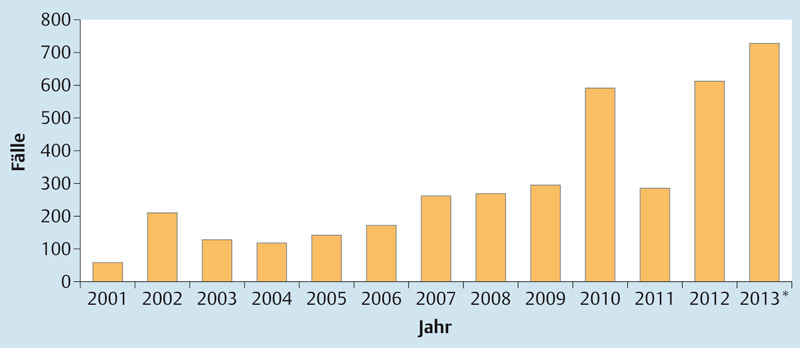
\includegraphics[scale=0.5]{Images/infektionszahlen_dengue_virus_deutschland.jpeg}
  \caption{\citetitle{cramer_dengue-virus_2014} \cite{cramer_dengue-virus_2014}}
  \label{fig:Dengue_virus_infektionszahlen_deutschland}
\end{figure}

Es ist wichtig, die Mutationen der Virenfamilie zu untersuchen und Vorhersagen \"uber die Bereiche zu machen, in denen das Virus eher mutieren kann und wo eher nicht, da Viren, wie die Dengue-Viren, Meister darin sind, das Immunsystem des Menschen zu \"uberlisten. Durch Mutationen k\"onnen sie sich besser an neue Wirte und Umgebungen anpassen, was ihre Verbreitung erleichtert und die Bek\"ampfung erschwert \cite{cramer_dengue-virus_2014}\cite{janisch_klein_2017}. Das Verst\"andnis der Mutationsmuster hilft bei der epidemiologischen \"Uberwachung. Wenn bekannt ist, welche Bereiche des Virusgenoms stabil sind und welche zu Mutationen neigen, k\"onnen Gesundheitsbeh\"orden besser absch\"atzen, wann und wo neue Ausbr\"uche auftreten k\"onnten. Dies ist besonders wichtig in Regionen, in denen invasive Stechm\"uckenarten wie Aedes albopictus nachgewiesen wurden, die als Vektoren f\"ur verschiedene Viren dienen k\"onnen \cite{cramer_dengue-virus_2014}. Die F\"ahigkeit, Mutationen vorherzusagen, kann helfen, potenzielle Pandemien fr\"uhzeitig zu erkennen und Ma\ss{}nahmen zu ergreifen, bevor sich das Virus weit verbreitet \cite{janisch_klein_2017}. Durch die Identifikation stabiler und variabler Regionen des Virusgenoms k\"onnen stabilere Impfstoffe und gezieltere Therapien entwickelt werden. Bei der Entwicklung von Impfstoffen und Medikamenten ist es wichtig absch\"atzen zu k\"onnen, welche Teile des Virus mutieren, da Impfstoffe und antivirale Therapien oft auf spezifische Teile des Virus zielen. Wenn diese Teile mutieren, k\"onnen Impfstoffe und Medikamente weniger wirksam werden \cite{janisch_klein_2017}. 
Insgesamt erm\"oglicht die Untersuchung von Virusmutationen eine proaktive und gezielte Reaktion auf virale Bedrohungen, was entscheidend f\"ur den Schutz der \"offentlichen Gesundheit ist.

\section{Beitr\"age dieser Arbeit}
% In a German thesis write: \section{Beiträge dieser Arbeit}

% !!!!!!!!!!!!!!!!!!!!!!!!!!!!!!!!!!
% !!! Your action is needed here !!!
% !!!!!!!!!!!!!!!!!!!!!!!!!!!!!!!!!!
%
% Replace with a detailed account of your contributions:


\section{Verwandte Arbeiten}
% In a German thesis write: \section{Verwandte Arbeiten}

% !!!!!!!!!!!!!!!!!!!!!!!!!!!!!!!!!!
% !!! Your action is needed here !!!
% !!!!!!!!!!!!!!!!!!!!!!!!!!!!!!!!!!
%
% Replace with a detailed account of what other people have already
% researched concerning your thesis's theme. Even when (indeed,
% especially when) there has been only little or even no research by
% other people, you should explain in detail that this is the case and
% why it is the case. 


\section{Aufbau dieser Arbeit}
% In a German thesis write: \section{Aufbau dieser Arbeit}


% !!!!!!!!!!!!!!!!!!!!!!!!!!!!!!!!!!
% !!! Your action is needed here !!!
% !!!!!!!!!!!!!!!!!!!!!!!!!!!!!!!!!!
%
% Replace the following by one or two paragraphs describing the
% thesis's structure.



% !!!!!!!!!!!!!!!!!!!!!!!!!!!!!!!!!!
% !!! Your action is needed here !!!
% !!!!!!!!!!!!!!!!!!!!!!!!!!!!!!!!!!
%
% Replace the whole text chapter with the main text of your thesis! 


\chapter{Material und Methoden}%: Document Setup and Document Structure}
\label{chapter-use}

\section{Dengue-Virus}
Serotypen sind Untergruppen von Mikroorganismen, wie Viren oder Bakterien, die sich durch spezifische antigenetische Eigenschaften unterscheiden. Diese Unterschiede beziehen sich auf die Struktur von Antigenen, die auf der Oberfl\"ache der Mikroben vorhanden sind. Serotypen k\"onnen durch serologische Tests identifiziert werden, bei denen Antik\"orper verwendet werden, um die Reaktion auf bestimmte Antigene zu bestimmen. Im Kontext von Viren, wie den Dengue-Viren, beziehen sich Serotypen auf die vier verschiedenen Varianten (DENV-1 \cite{tittarelli_dengue_2014}, DENV-2 \cite{cao_retrospective_2023}, DENV-3 \cite{peyrefitte_genetic_2003} und DENV-4 \cite{wardhani_genetic_2023}), die unterschiedliche immunologische Reaktionen hervorrufen k\"onnen. In dieser Arbeit schauen wir uns alle vier Serotypen an, um Mutationen zwischen den verschiedenen Serotypen untersuchen zu k\"onnen. 
Dengue-Viren sind umh\"ullte, positive-Strang-RNA-Viren, die zur Familie der Flaviviridae geh\"oren. Der Virusk\"orper besteht aus einer Lipid-Doppelschicht, die von Membran- (M) und H\"ullproteinen (E) umgeben ist. Im Inneren befindet sich das Nukleokapsid, das aus dem Kapsidprotein (C) und dem Genom-RNA-Strang zusammengesetzt ist. Die H\"ullproteine (E) sind Typ-II-Transmembranproteine, die aus einer N-terminalen Ektodom\"ane, einer Transmembrandom\"ane und einer C-terminalen zytoplasmatischen Dom\"ane bestehen. Die Ektodom\"ane ist f\"ur die Bindung an Wirtszellrezeptoren und die Fusion mit der Wirtszellmembran verantwortlich. Die Transmembrandom\"ane verankert das E-Protein in der Virush\"ulle und durchspannt die Lipid-Doppelschicht. Die kurze zytoplasmatische Dom\"ane interagiert mit dem Kapsidprotein. Die Membranproteine (M) sind ebenfalls Typ-II-Transmembranproteine, die aus einer N-terminalen Ektodom\"ane, einer Transmembrandom\"ane und einer C-terminalen zytoplasmatischen Dom\"ane aufgebaut sind. Sie sind an der Reifung und Freisetzung infekti\"oser Viruspartikel beteiligt. Beide Transmembranproteine, E und M, durchspannen die Lipid-Doppelschicht der Virush\"ulle mit ihren hydrophoben Transmembrandom\"anen. Diese Dom\"anen sind f\"ur die Verankerung und Stabilit\"at der Proteine in der Membran von entscheidender Bedeutung. Mutationen in diesen Regionen k\"onnen die Faltung, Insertion und Stabilit\"at der Proteine beeinflussen und somit die Infektiosit\"at und \"Uberlebensf\"ahigkeit des Virus beeintr\"achtigen. Dengue-Viren besitzen au\ss{}erdem einige nicht-strukturelle Proteine, die f\"ur den Lebenszyklus des Virus entscheidend sind. Die wichtigsten Proteine, die in diesem Zusammenhang erw\"ahnt werden, sind: 2K, NS1, NS2A, NS2B, NS3, NS4A, NS4B und NS5. 2K ist ein kleines Protein, das als Transmembranprotein fungiert und eine Rolle bei der Virusreifung spielt. NS1 ist ein wichtiges virales Glycoprotein, das in der Zelle sekretiert wird und an der Virusreplikation beteiligt ist. Es hat keine transmembrane Region, sondern ist haupts\"achlich im Zytoplasma und im Extrazellul\"arraum aktiv. NS2A ist ein kleines, hydrophobes Protein, das als Transmembranprotein wirkt und an der Membran des endoplasmatischen Retikulums lokalisiert ist. Es spielt eine Rolle bei der Virusreplikation und der Modifikation der Wirtszellmembran. NS2B ist ein Co-Faktor f\"ur die Protease NS3 und hat eine transmembrane Region, die es in die Membran des endoplasmatischen Retikulums einbettet. NS3 ist ein wichtiges Enzym, das als Serinprotease und RNA-Helikase fungiert. Es hat eine transmembrane Region, die es in die Membran integriert. NS4A ist ebenfalls ein Transmembranprotein und spielt eine Rolle in der Virusreplikation und der Modulation der Wirtszellantwort. NS4B ist ein weiteres Transmembranprotein, das an der Virusreplikation beteiligt ist und in der Membran des endoplasmatischen Retikulums lokalisiert ist. NS5 ist das gr\"o\ss{}te Protein des Dengue-Virus, das als RNA-abh\"angige RNA-Polymerase fungiert. Es hat auch eine transmembrane Region, die es in die Membran einbettet.
Insgesamt sind die Transmembranproteine im Dengue-Virus: E, M, 2K, NS2A, NS2B, NS3, NS4A, NS4B und NS5. Wobei NS2A fast vollst\"andig in der Membran verankert liegt. Der Aufbau des Dengue-Virus und die transmembranen Regionen sind in der Abbildung \ref{fig:Dengue_virus_overview} aus dem Paper \citetitle{perera_structural_2008} von \citeauthor{perera_structural_2008} \cite{perera_structural_2008} visualisiert. \\
\begin{figure}[htpb]
  \centering
  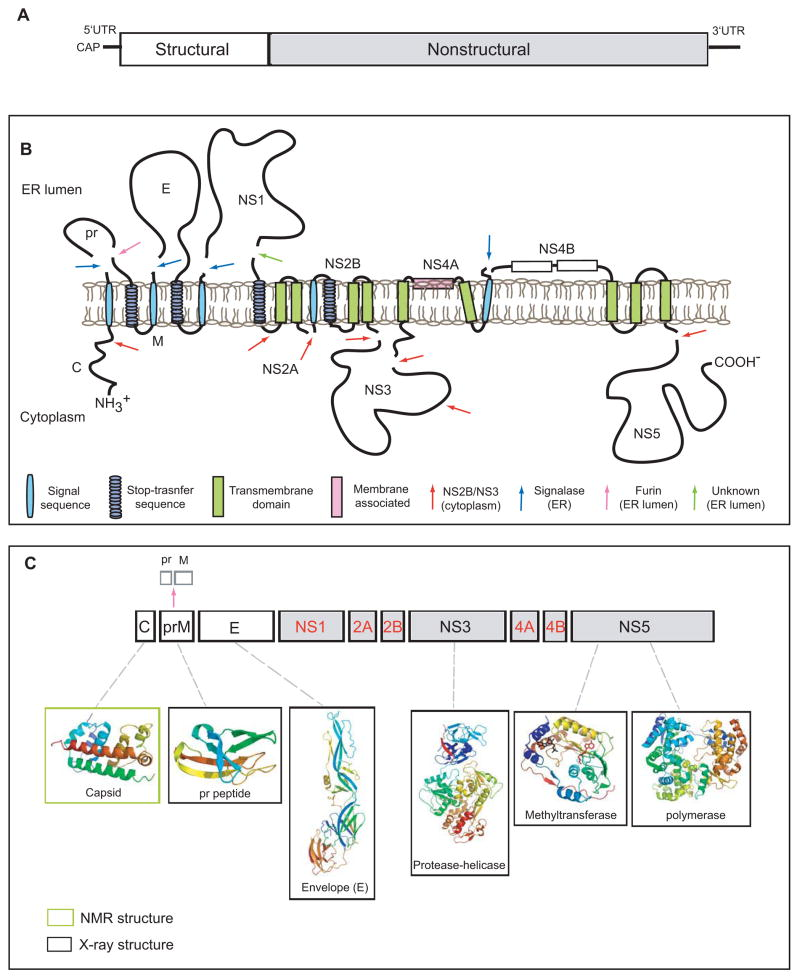
\includegraphics[scale=1]{Images/Dengue_virus_overview.jpg}
  \caption{\citetitle{perera_structural_2008} \cite{perera_structural_2008}}
  \label{fig:Dengue_virus_overview}
\end{figure} 

Die Untersuchung der Transmembranproteine im Dengue-Virus bietet nicht nur Einblicke in deren strukturelle Eigenschaften, sondern \"offnet auch den Weg zu einem tiefergehenden Verst\"andnis der Wechselwirkungen zwischen diesen Proteinen und ihrer Umgebung. Insbesondere die hydrophoben und hydrophilen Bereiche der Transmembranregionen spielen eine entscheidende Rolle f\"ur die Stabilit\"at und Funktionalit\"at der Proteine. Um die spezifischen Eigenschaften dieser Bereiche zu quantifizieren, ist es notwendig, die Konzepte der polar requirements und der Hydropathie zu betrachten. Diese Konzepte erm\"oglichen es, die hydrophilen und hydrophoben Eigenschaften der Aminos\"auresequenzen zu messen und zu analysieren, was f\"ur das Verst\"andnis der Interaktionen zwischen den transmembren Bereichen und ihrer Umgebung von zentraler Bedeutung ist.

\section{Hydropathie und polar requirements}
Hydropathie beschreibt die Affinit\"at eines Molek\"uls zu Wasser. Molek\"ule k\"onnen als hydrophil (wasserliebend) oder hydrophob (wasserabweisend) klassifiziert werden. Diese Eigenschaften beeinflussen, wie Molek\"ule in biologischen Systemen interagieren, insbesondere in Bezug auf Proteine und deren Funktion. Hydropathie wird besonders h\"aufig verwendet, um eine bestimmte Untergruppe von Proteinen, die Membranproteine, zu untersuchen. Diese liegen teilweise in der Membran und k\"onnen transmembrane Regionen besitzen, wo das Protein die Membran einmal vollst\"andig durchzieht. Jedes Molek\"ul hat ein charakteristisches Hydropathie-Profil, das als eine Art "`Fingerabdruck"' f\"ur seine Struktur betrachtet werden kann. Diese Profile werden h\"aufig verwendet, um die Struktur und Funktion von Membranproteinen zu analysieren und um Beziehungen zwischen verschiedenen Transportproteinen zu identifizieren. In biologischen Systemen spielen hydrophobe und hydrophile Wechselwirkungen eine entscheidende Rolle bei der Faltung von Proteinen, der Bildung von Zellmembranen und der Funktion von Enzymen. Das Verst\"andnis dieser Eigenschaften hilft bei der Vorhersage, wie Molek\"ule in zellul\"aren Umgebungen interagieren. Hydropathie-Analysen werden in der Bioinformatik und Strukturbiologie eingesetzt, um die Topologie von Membranproteinen vorherzusagen und deren funktionelle Eigenschaften besser zu verstehen. Zusammenfassend ist die Hydropathie eine grundlegende chemische Eigenschaft, die entscheidend f\"ur das Verst\"andnis der Molek\"ulinteraktionen in biologischen Systemen ist. Da sie die grundlegenden Molek\"uleigenschaften des Proteins beschreibt. 
Somit hat auch jede Aminos\"aure einen spezifischen Hydropathiewert. In dieser Arbeit verwenden wir die Werte aus dem Paper \citetitle{kyte_simple_1982} von \citeauthor{kyte_simple_1982} \cite{kyte_simple_1982}. Die in der Abbildung \ref{fig:Hydropathieindexe} zu sehen sind. Die Hydropathie-Indizes, wie sie von \citeauthor{kyte_simple_1982} entwickelt wurden, quantifizieren die hydrophoben und hydrophilen Eigenschaften von Aminos\"auren in Proteinen. Diese Indizes basieren auf der Messung der Energie, die erforderlich ist, um eine Aminos\"aure aus einer w\"assrigen L\"osung in eine hydrophobe Umgebung zu transferieren. Im Wesentlichen wurde f\"ur jede Aminos\"aure ein Wert zugewiesen, der ihre Neigung beschreibt, sich in w\"assriger Umgebung zu l\"osen oder in einer hydrophoben Phase zu verbleiben. Die Werte reichen von stark negativ (sehr hydrophil) bis stark positiv (sehr hydrophob).
\begin{figure}[htpb]
  \centering
  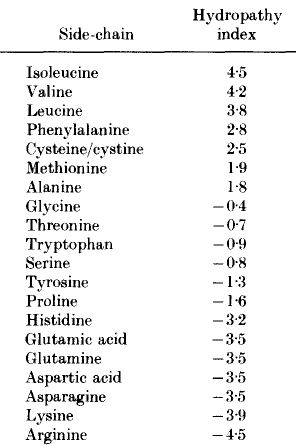
\includegraphics[scale=0.75]{Images/Hydropathy_scores_Paper.png}
  \caption{Aminos\"auren mit zugeh\"origen Hydropathieindexen aus \citetitle{kyte_simple_1982} \cite{kyte_simple_1982}}
  \label{fig:Hydropathieindexe}
\end{figure}
In dem Paper \citetitle{kyte_simple_1982} \cite{kyte_simple_1982} werden vier spezifische Werte des Hydropathie-Index manuell angepasst. Diese Anpassungen betreffen die Aminos\"auren Glycin, Alanin, Serin und Threonin. Die Gr\"unde f\"ur diese \"Anderungen sind, dass die Autoren die Hydropathie-Indexe dieser Aminos\"auren so modifizieren wollten, dass sie besser die experimentellen Beobachtungen und die biologischen Eigenschaften der Proteine widerspiegeln.

Im chemischen Kontext beziehen sich "`polar requirements"' auf die spezifischen Eigenschaften und Bedingungen, die f\"ur polare Molek\"ule oder chemische Verbindungen erforderlich sind, um in einer bestimmten Umgebung stabil zu sein oder zu interagieren. Diese Anforderungen k\"onnen die Polarit\"at, L\"oslichkeit, Wechselwirkungen mit anderen Molek\"ulen und die F\"ahigkeit zur Bildung von Wasserstoffbr\"ucken umfassen. Molek\"ule mit polaren Gruppen (z. B. Hydroxyl- oder Carboxylgruppen) haben unterschiedliche Eigenschaften im Vergleich zu unpolaren Molek\"ulen. Die Polarit\"at beeinflusst, wie Molek\"ule in L\"osungsmitteln interagieren, insbesondere in w\"assrigen L\"osungen. Polare Molek\"ule sind in polaren L\"osungsmitteln wie Wasser besser l\"oslich. Die polar requirements helfen zu bestimmen, welche Molek\"ule in bestimmten chemischen Reaktionen oder biologischen Prozessen effektiv interagieren k\"onnen. Die polar requirements sind entscheidend f\"ur die Vorhersage von Wechselwirkungen zwischen Molek\"ulen, wie z. B. zwischen Enzymen und Substraten oder zwischen Rezeptoren und Liganden. In der Biochemie sind die polar requirements wichtig f\"ur das Verst\"andnis der Struktur und Funktion von Biomolek\"ulen, einschlie\ss{}lich Proteinen und Nukleins\"auren. Auch polar requirements sind entscheidend f\"ur das grundlegende Verst\"andnis der Molek\"uleigenschaften eines Proteins. 
Aminos\"auren haben spezifische polar requirements Werte. In dieser Arbeit nutzen wir die Werte aus der Arbeit \citetitle{woese_fundamental_1966} von \citeauthor{woese_fundamental_1966} \cite{woese_fundamental_1966}. Die in der Abbildung \ref{fig:Polar_requirements_indexe} zu sehen sind. 
\begin{figure}[htpb]
  \centering
  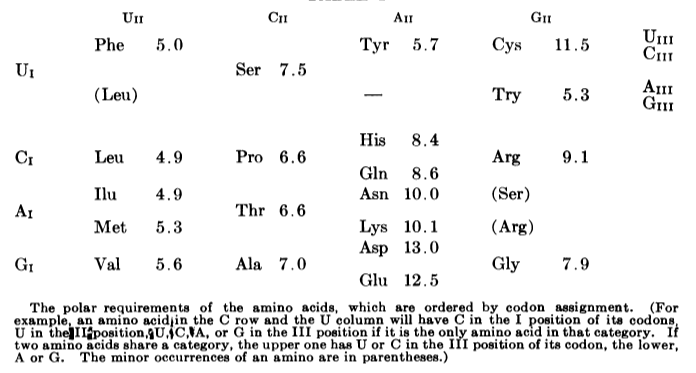
\includegraphics[scale=0.6]{Images/polar_requirements_scores_Paper.png}
  \caption{Aminos\"auren mit zugeh\"origen Polar requirements Werten aus \citetitle{woese_fundamental_1966} \cite{woese_fundamental_1966}}
  \label{fig:Polar_requirements_indexe}
\end{figure}
Die Polar-Requirements-Werte, wie sie von \citeauthor{woese_fundamental_1966} eingef\"uhrt wurden, geben an, wie stark eine Aminos\"aure polare Wechselwirkungen eingeht. Diese Werte wurden durch die Messung der freien Enthalpie berechnet, die erforderlich ist, um eine Aminos\"aure von einer unpolaren in eine polare Umgebung zu transferieren. Die polar requirements Werte wurden in einem Experiment bestimmt, bei dem die L\"oslichkeit jeder Aminos\"aure in Wasser und einem unpolaren L\"osungsmittel gemessen wurde. Konkret verwendeten sie Octanol als unpolare Phase. Das Experiment lief folgenderma\ss{}en ab: F\"ur jede der 20 proteinogenen Aminos\"auren wurde die L\"oslichkeit in Wasser und Octanol bestimmt. Dazu wurde eine definierte Menge der Aminos\"aure in beide L\"osungsmittel gegeben und die Konzentration in der jeweiligen Phase gemessen. Aus dem Unterschied in der L\"oslichkeit konnte dann die freie Enthalpie f\"ur den Transfer zwischen den beiden Phasen berechnet werden. Je gr\"o\ss{}er der Wert, desto st\"arker die Tendenz der Aminos\"aure, polare Wechselwirkungen einzugehen und sich in einer w\"assrigen Umgebung aufzuhalten. Die Werte reichen von sehr niedrig (unpolar) bis sehr hoch (polar). Sie erm\"oglichen es, die Aminos\"auren nach ihrer Polarit\"at zu ordnen und R\"uckschl\"usse auf die Oberfl\"achenexposition und Interaktionen von Proteinen zu ziehen. In Kombination mit anderen Parametern wie den Hydropathie-Indizes liefern sie wertvolle Informationen f\"ur die Strukturvorhersage und das Proteindesign.

Obwohl Hydropathie und polar requirements \"ahnliche Eigenschaften untersuchen, zeigt sich bei den Werten einige Unterschiede. Da nicht alle Aminos\"auren einduetig zu klassifiezieren sind, wenn man nur eine der beiden Molek\"uleigenschaften verwendet und somit wertvolle Information \"uber die Struktur des Proteins verloren geht. Aus diesem Grund verwenden wir beide Werte f\"ur die Berechnung. 

\section{Biopython}
In dieser Arbeit wurde Biopython, eine Sammlung von Python-Bibliotheken f\"ur die Bioinformatik, verwendet, um die Datenanalyse durchzuf\"uhren. Biopython erm\"oglicht die einfache Handhabung von biologischen Datenformaten und die Durchf\"uhrung komplexer bioinformatischer Analysen. Das Modul SeqIO wurde in dieser Arbeit verwendet, um Sequenzen einzulesen. 

\section{T-Coffee}
T-Coffee (Tree-based Consistency Objective Function for Alignment Evaluation) ist ein in der Bioinformatik weit verbreitetes Werkzeug zur Ausrichtung von DNA-, RNA- und Proteinsequenzen. T-Coffee arbeitet mit einer Ausrichtungsstrategie in Kombination mit einer konsistenzbasierten Bewertungsfunktion. Der Algorithmus f\"ur T-Coffee wird haupts\"achlich in der Originalver\"offentlichung \citetitle{poirot_tcoffeeigs_2003} \cite{poirot_tcoffeeigs_2003} beschrieben. Der Algorithmus hat die folgenden Hauptschritte. Zun\"achst generiert T-Coffee alle m\"oglichen paarweisen Ausrichtungen zwischen den Eingabesequenzen unter Verwendung globaler und lokaler Ausrichtungsmethoden. Anschlie\ss{}end erstellt es eine prim\"are Bibliothek mit Ausrichtungsinformationen aus diesen paarweisen Ausrichtungen und weist jedem ausgerichteten Residuenpaar basierend auf seiner Konsistenz \"uber verschiedene Ausrichtungen hinweg Gewichte zu. Die prim\"are Bibliothek wird durch Einbeziehung transitiver Ausrichtungen erweitert, was hilft, indirekte Beziehungen zwischen Sequenzen zu erfassen. Unter Verwendung der erweiterten Bibliothek konstruiert T-Coffee einen F\"uhrungsbaum und f\"uhrt eine progressive Ausrichtung durch, wobei zun\"achst die \"ahnlichsten Sequenzen ausgerichtet und dann nach und nach entferntere Sequenzen hinzugef\"ugt werden. Die anf\"angliche Ausrichtung wird iterativ verfeinert, um ihre Gesamtqualit\"at und -konsistenz zu verbessern.
T-Coffee zeichnet sich durch seine hohe Genauigkeit aus, insbesondere bei der Bearbeitung kurzer Sequenzen. Es wurde mit anderen Ausrichtungswerkzeugen verglichen und hat gezeigt, dass es Ausrichtungen mit einer Genauigkeit produziert, die mit anderen Methoden wie MUSCLE \cite{Edgar2004MUSCLEL} vergleichbar oder besser ist.

\section{Berechnungsgrundlagen}
In den folgenden Diagrammen schauen wir uns das Polyprotein des Dengue-Virus an und teilen daf\"ur das Protein in 20 gleich gro\ss{}e Abschnitte auf. F\"ur diese Abschnitte f\"uhren wir die Berechnungen jeweils durch und stellen die einzelnen Ergebnisse dann in einer Grafik gemeinsam dar. Die Serotypen wurden hierf\"ur zuerst mit T-Coffee ausgerichtet. Dadurch waren alle Sequenzen gleich lang und konnten somit in gleich gro\ss{}e Bereiche aufgeteilt werden. Im Folgenden ist von einzelnen Stellen der Sequenzen die Rede; dabei ist gemeint, dass man sich in dem Alignment an einer Stelle alle Sequenzen anschaut. 

Um die Mutationen zu z\"ahlen, schauen wir f\"ur alle Sequenzen, an einer Stelle, ob alle Aminos\"auren gleich sind oder ob es mindestens eine Sequenz gibt, in der es eine andere Aminos\"aure an dieser Stelle gibt. Wenn ein Gap an der Stelle existiert, wird das auch als Mutation gez\"ahlt. Wir gehen dabei \"uber die gesamte L\"ange der Sequenzen und z\"ahlen alle Stellen, an der wir mindestens zwei verschiedene Aminos\"auren oder ein Gap vorfinden. Wir z\"ahlen expliziet nicht, wie viele verschiedene Aminos\"auren es an dieser Stelle gibt. Wenn wir also eine Mutation z\"ahlen, meinen wir, dass an der jeweiligen Stelle mindestens eine Sequenz eine andere Aminos\"aure aufweist, als die Aminos\"aure in der ersten Sequenz oder ein Gap an dieser Stelle besitzt. In den folgenden Grafiken, nutzen wir au\ss{}erdem nur den Anteil an Mutationen \"uber einen Sequenzteil. Wir berechen die Anzahl an Mutationen daf\"ur anteilig f\"ur die L\"ange der jeweiligen Sequenz. Wir berechnen also, verh\"altnism\"a\ss{}ig, an wie vielen Stellen die Sequenz mutiert ist. F\"ur das Polyprotein des Dengue-Virus ergibt sich dadurch die Abbildung \ref{fig:Dengue_virus_mutations}. 
\begin{figure}[htpb]
  \centering
  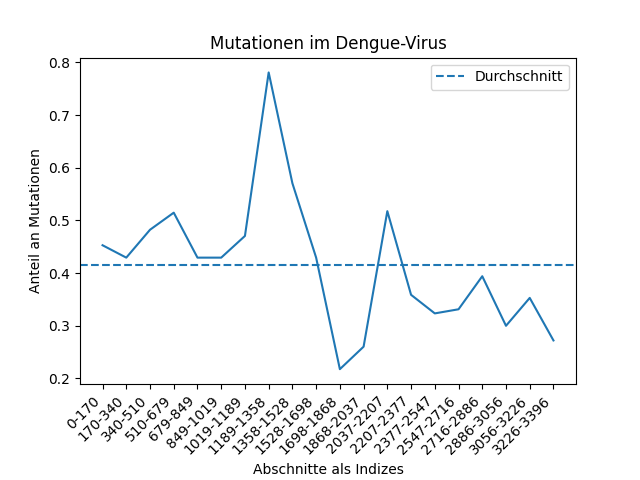
\includegraphics[scale=0.75]{Images/Diagramm_Mutationen_im_Dengue_virus.png}
  \caption{Mutationen im Dengue-Virus}
  \label{fig:Dengue_virus_mutations}
\end{figure}

Im n\"achsten Schritt wird f\"ur jede Stelle der Sequenzen der minimale und der maximale Wert ausgerechnet, den die Aminos\"auren in Bezug auf polar requirements zugeordnet bekommen. Wir nutzen hierf\"ur die Werte aus der Abbildung \ref{fig:Polar_requirements_indexe} als Grundlage, um den Aminos\"auren Werte zuzuordnen. Wir normieren die Werte vor den weiteren Berechnungsschritten noch auf einen Wertebereich zwischen 0 und 1. Gaps haben keine zugeordneten Werte und werden somit bei der Berechnung der polar requirements nicht beachtet. Wir berechnen nun die Differenz zwischen dem maximalen und minimalen Wert an der jeweiligen Stelle. Da wir die Werte voher normiert haben, ist die maximale Differenz zwischen den Aminos\"auren 1 und die minimale 0. Insgesamt berechnen wir f\"ur jede Stelle einer Teilsequenz diese Differenzen und addieren sie auf, damit wir f\"ur eine Teilsequenz dann mithilfe der L\"ange der Teilsequenz den Durschnitt der Differenzen berechnen k\"onnen. Der polar requirements Wert f\"ur eine Teilsequenz ist somit die durchschnittliche Differenz des maximalen und minimalen normierten Wertes an jeder Stelle der Teilsequenz. F\"ur das Polyprotein des Dengue-Virus ergibt sich dadurch folgende Abbildung \ref{fig:Dengue_virus_polar_requirements}. 
\begin{figure}[htpb]
  \centering
  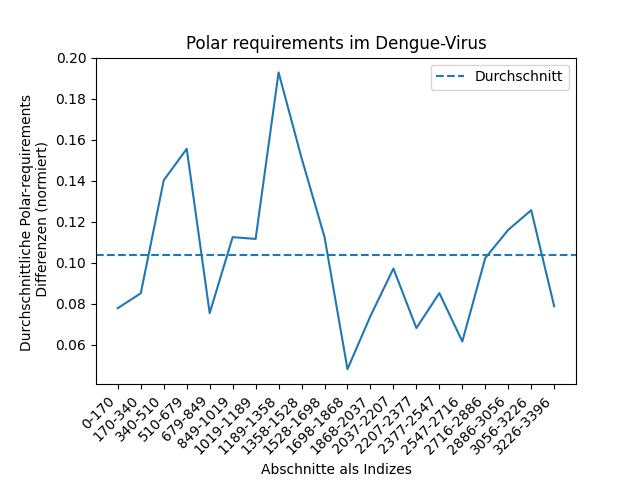
\includegraphics[scale=0.75]{Images/Diagramm_Polar_requirements_im_Dengue_virus.png}
  \caption{Polar requirements im Dengue-Virus}
  \label{fig:Dengue_virus_polar_requirements}
\end{figure}

F\"ur Hydropathie berechnen wir die Werte gleicherma\ss{}en. Wir nutzen daf\"ur die Werte aus der Abbildung \ref{fig:Hydropathieindexe} und berechnen die Werte auf die selbe Weise wie bei den polar requirements. Gaps werden hier auch wieder nicht ber\"ucksichtigt. Wir berechnen also die durchschnittliche Differenz des maximalen und minimalen normierten Wertes an jeder Stelle der Teilsequenz. F\"ur das Polyprotein des Dengue-Virus ergibt sich dadurch folgende Abbildung \ref{fig:Dengue_virus_hydropathy}. 
\begin{figure}[htpb]
  \centering
  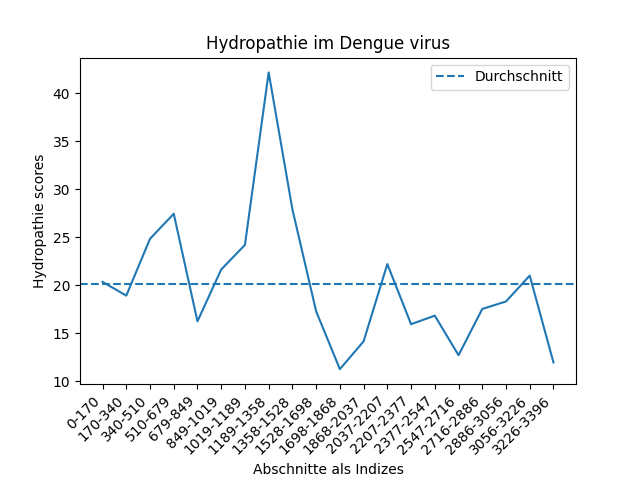
\includegraphics[scale=0.75]{Images/Diagramm_Hydropathie_im_Dengue_virus.png}
  \caption{Hydropathie im Dengue-Virus}
  \label{fig:Dengue_virus_hydropathy}
\end{figure}

Um einen gemeinsamen Score zu bilden, werden nun die Werte f\"ur polar requirements und Hydropathie f\"ur eine Teilsequenz gemittelt. Der Score ist also der Durchschnitt \"uber die durchschnittlichen Differenzen des maximalen und minimalen Wertes f\"ur Hydropathie und polar requirements an jeder Stelle der Teilsequenz. F\"ur das Polyprotein des Dengue-Virus ergibt sich dadurch folgende Abbildung \ref{fig:Dengue_virus_scores}. 
\begin{figure}[htpb]
  \centering
  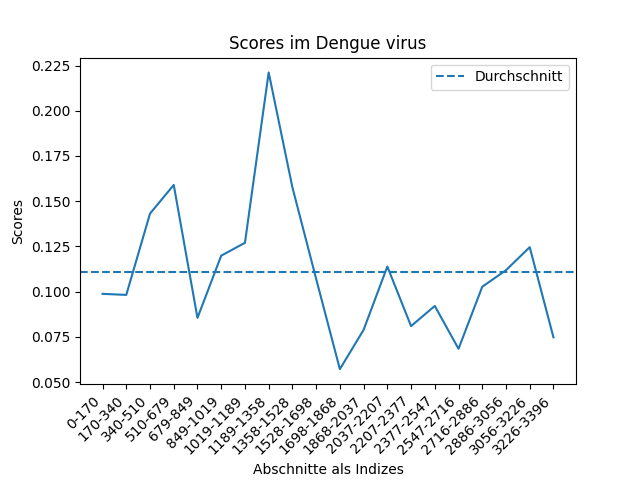
\includegraphics[scale=0.75]{Images/Diagramm_Scores_im_Dengue_virus.png}
  \caption{Scores im Dengue-Virus}
  \label{fig:Dengue_virus_scores}
\end{figure}

Die Abbildung \ref{fig:Dengue_virus_scores_and_mutations_bereiche} kombiniert den gemeinsamen Score und den Anteil an Mutationen in einem Diagramm. 
\begin{figure}[htpb]
  \centering
  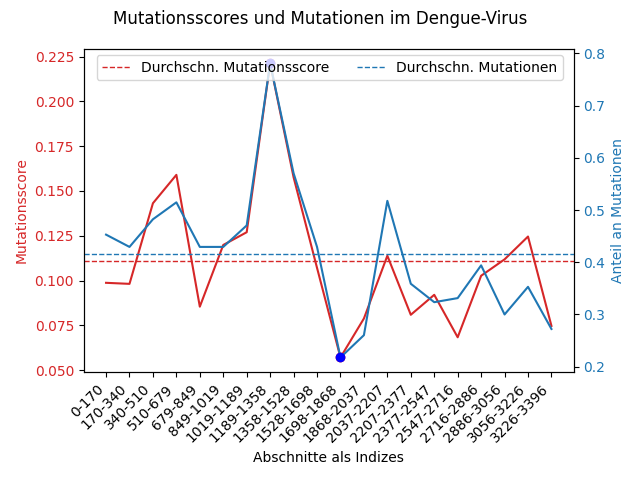
\includegraphics[scale=0.75]{Images/Diagramm_Scores_und_Mutationen_Dengue_viren_Bereiche.png}
  \caption{Diagramm: Scores und Mutationen Dengue-Viren: automatische Auteilung der Sequenzen in 20 gleich gro\ss{}e Bereiche}
  \label{fig:Dengue_virus_scores_and_mutations_bereiche}
\end{figure}

Die Abbildung \ref{fig:Dengue_virus_scores_and_mutations_bereiche_random} folgt den gleichen Berechnungen wie die Abbildung \ref{fig:Dengue_virus_scores_and_mutations_bereiche}. F\"ur diese Abbildung nutzen wir jedoch nicht das Polyprotein des Dengue-Virus in normaler Form, sondern ver\"andern die Sequenzen, bevor wir die Scores und Mutationen berechnen. Wir erstellen eine zuf\"allige Permutation des Dengue-Viruses, indem wir eine Stelle des Alignments aller Serotypen zuf\"allig ausw\"ahlen und mit einer anderen zuf\"alligen Stelle vertauschen. Das Alignment bleibt also prinzipiell erhalten, und es werden nur einzelne Stellen des Alignments an eine andere Position im Alignment vertauscht. F\"ur die Abbildung \ref{fig:Dengue_virus_scores_and_mutations_bereiche_random} wurden 1000 zuf\"allige Vertauschungen nacheinander durchgef\"uhrt. Es kann also auch eine Stelle mehrfach vertauscht werden. 
\begin{figure}[htpb]
  \centering
  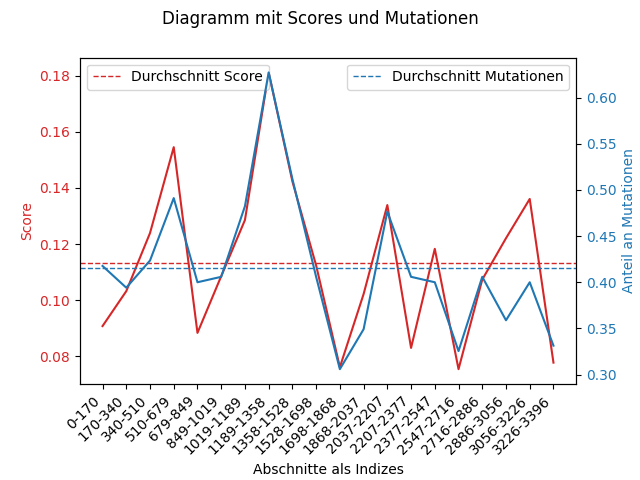
\includegraphics[scale=0.75]{Images/Diagramm_Scores_und_Mutationen_Dengue_viren_Bereiche_random.png}
  \caption{Diagramm: Scores und Mutationen Dengue-Viren: automatische Auteilung der Sequenzen in 20 gleich gro\ss{}e Bereiche mit zuf\"alliger Permutation des Dengue-Viruses mit 1000 Vertauschungen}
  \label{fig:Dengue_virus_scores_and_mutations_bereiche_random}
\end{figure}

Die Abbildung \ref{fig:Dengue_virus_scores_and_mutations_namen} benutzt auch die gleichen Berechnungen wie die Abbildung \ref{fig:Dengue_virus_scores_and_mutations_bereiche}. Hierbei wurden jedoch die Sequenzteile f\"ur die Berechnung ver\"andert. W\"ahrend bei den bisherigen Abbildungen gleich gro\ss{}e Bereiche ausgew\"ahlt werden, werden in dieser Abbildung verschieden gro\ss{}e Bereiche berechnet. Wir betrachten jedes Protein des Polyproteins einzeln und berechnen f\"ur jedes Protein einen Score und den Anteil an Mutationen. Daf\"ur suchen wir zuerst die betreffenden Regionen im Polyprotein f\"ur jeden Serotypen und erstellen dann ein Alignment mithilfe von T-Coffee, explizit f\"ur diese Region, um dann basierend auf diesem Alignment einen Score und den Anteil an Mutationen zu berechnen. Da die Proteine nicht alle die gleiche L\"ange haben, sind die betrachteten Bereiche nun unterschiedlich gro\ss{}. Da jedoch beide berechneten Werte anteilig in Bezug auf die L\"ange berechnet werden, bleiben die Werte vergleichbar miteinander. 
\begin{figure}[htpb]
  \centering
  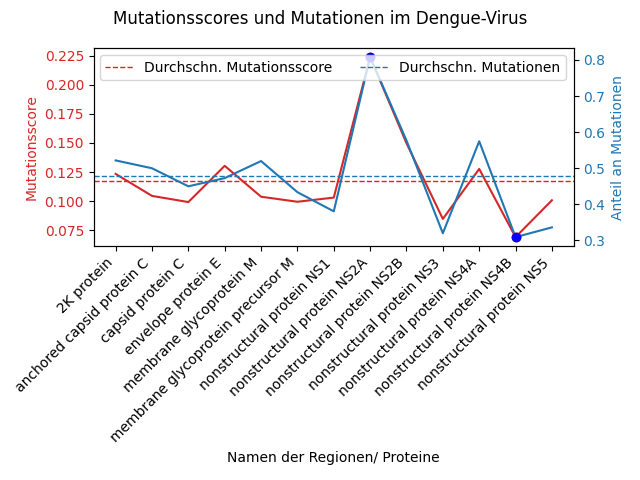
\includegraphics[scale=0.75]{Images/Diagramm_Scores_und_Mutationen_Dengue_viren_Namen.png}
  \caption{Diagramm: Scores und Mutationen Dengue-Viren: Auteilung nach Proteinen/ Bereichen}
  \label{fig:Dengue_virus_scores_and_mutations_namen}
\end{figure}

\chapter{Ergebnisse}
In der Abbildung \ref{fig:Dengue_virus_scores_and_mutations_bereiche} sind starke Abweichungen von den durchschnittlichen Werten f\"ur den Score und den Anteil an Mutationen zu erkennen. Insbesondere bei den Abschnitten 1189-1358 und 1698-1868 ist ein Maximum beziehungsweise ein Minimum zu erkennen. Um zu sch\"atzen, ob diese Extrema signifikant sind und nicht nur zuf\"alligen Schwankungen unterliegen, betrachten wir die Abbildung \ref{fig:Dengue_virus_scores_and_mutations_bereiche_random}. Hier wurde die Sequenz zuf\"allig permutiert. Wenn die Extrema zuf\"allige Schwankungen sind, k\"onnen wir annehmen, dass, wenn wir die Sequenz zuf\"allig stellenweise vertauschen, dass dann Extrema weiterhin im selben Ausma\ss{} vorkommen. Wenn die Extrema nicht auf Zufall basieren, sollten die Extrema in der zuf\"allig permutierten Sequenz abgeschw\"acht vorkommen. Die Werte sollten sich also dem Durchschnitt ann\"ahern, da die starken H\"aufungen von Mutationen oder die starken regionalen Ver\"anderungen im Score abgeschw\"acht wurden, indem einzelne Stellen aus diesem Bereich mit Stellen aus anderen Bereichen der Sequenz, in denen weniger Mutationen oder gro\ss{}e Differenzen im Score zu finden sind, vertauscht wurden. Da die Vertauschungen jedoch zuf\"allig ausgef\"uhrt wurden, existiert kein Bias dar\"uber, welche Stellen ausgew\"ahlt und vertauscht wurden. Sollten die Extrema also zuf\"allig entstanden sein, sollten sich nun an einigen Stellen in der Sequenz wieder geh\"auft Mutationen finden lassen oder starke Ver\"anderungen im Score bestehen. 
Zu erkennen in der Abbilung \ref{fig:Dengue_virus_scores_and_mutations_bereiche_random} ist, dass der Bereich \"uber den sich die Werte erstrecken verkleinert ist, im Vergleich zur Abbildung \ref{fig:Dengue_virus_scores_and_mutations_bereiche}. Bei der Abbildung \ref{fig:Dengue_virus_scores_and_mutations_bereiche_random} sind f\"ur die Scores Werte im Bereich von circa 0,0582 bis 0,2299 zu erkennen und f\"ur den Anteil an Mutationen Werte im Bereich von circa 0,2176 bis 0,7811. Bei der Abbildung \ref{fig:Dengue_virus_scores_and_mutations_bereiche} sind f\"ur den Score Werte im Bereich von circa 0,0826 bis 0,1778 zu erkennen und f\"ur den Anteil an Mutationen Werte im Bereich von circa 0,3195 bis 0,6036. Die Extrema sind also abgeschw\"acht, wodurch anzunehmen ist, dass die Extrema nicht nur zuf\"allig entstanden sind. Deshalb nehmen wir an, dass die Ergebnisse auch signifikant sind, da die Werte nicht nur zuf\"alligen Schwankungen unterliegen.  

Um die Fragestellung zu beantworten betrachten wir die Abbildung \ref{fig:Dengue_virus_scores_and_mutations_namen}. Hierbei f\"allt direkt auf, dass die Proteine NS2A, NS3 und NS4B besonders extreme Werte aufweisen, sowohl bei dem Score als auch bei dem Anteil an Mutationen. Das Protein NS2A hat dabei besonders hohe Werte, weshalb davon auszugehen ist, dass kein besonders starker Konservierungsdruck in diesem Protein vorhanden sein kann, sondern das Protein eher einem gro\ss{}en Mutationsdruck unterliegt und besonders h\"aufig mutiert. Die Proteine NS3 und NS4B weisen hingegen besonders niedrige Werte auf, sodass von einem starken Konservierungsdruck und einem sehr niedrigem Mutationsdruck innerhalb der Proteine ausgegangen werden kann. 


\chapter{Diskussion}
- NS2A nicht wie erwartet hoch konserviert (gr\"o\ss{}tenteils in der Membran liegend) -> ist ein Protein, was aber h\"aufig Mutieren muss, besitzt somit Mutationsdruck (auf andere Quellen verlinken, die das zeigen und Funktionsweise erkl\"aren, mit verweis auf Mutationsdruck bez\"uglich des Ausweichens der Immunabwehr) \\
- NS3 und NS5 sind wie erwartet ausgeschlagen -> auch Membranproteine. \\
- Restlichen Proteine eher keine Informationen, weil sie auch zuf\"alligen Schwankungen unterliegen k\"onnten. \\
--> Somit Fragestellung irgendwie nicht zufriedenstellen Beantwortet -> NS2A aber definitiv nicht erf\"ullend -> eigentlich also Hypothese widerlegt, aber wait, was passiert, wenn man sich NS2A genauer anschaut und explizit darauf schaut, ob es auch wirklich genau in den TR-Regionen h\"aufig mutiert, oder eher au\ss{}erhalb der Membran -> 2. Fragestellung 

\chapter{Zusammenfassung und Ausblick}
% In a German thesis write: \subsection{Zusammenfassung und Ausblick}


% !!!!!!!!!!!!!!!!!!!!!!!!!!!!!!!!!!
% !!! Your action is needed here !!!
% !!!!!!!!!!!!!!!!!!!!!!!!!!!!!!!!!!
%
% Replace the following with your conclusion



% Normally, the bibliography comes next at this point. Do *not* (try
% to) include further indices and tables like an index or
% a list of figures or a list of tables or such things. Nobody
% actually uses them and they just use up space. 
%
% You *can* however include a glossary, if this seems appropriate. It
% goes here as an unnumbered chapter. Most thesis will *not* need a
% glossary: a well-written text (re)explains strange words and
% concepts as necessary. However, there are situations where a
% glossary may be helpful.














%%%
% 
% Bibliographies
%
%%%
%
% The uzl-thesis class will load biblatex for the bibliography
% management. This is a powerful package, see its documentation for
% details. The styles will be setup correctly and automatically by
% choosing one of the two style keys as described earlier.
%
% In order for the bibliography to work, run latex in the following
% order (which is the standard order):
% 
% > lualatex thesis-example
% > bibtex thesis-example
% > lualatex thesis-example
% 
% Add BibTeX files using \addbibresource or use the {bibtex entries}
% environment (see below).
%
%%%
%
% Although everyting is normally setup automatically, you can change
% the options passed to biblatex using the key 'biblatex';
% for instance,
%
%   \UzLThesisSetup{biblatex={firstinits=false}}
%
% will switch off shortened first names. Normally, you will not need
% this key in your preamble. 
% 
% Note that the bibtex program is used as the 'backend' of biblatex
% by default (rather than biber, which is the preferred program of
% biblatex). This means that you can (and must) run *bibtex* after you
% have run lualatex on your thesis. If you wish to use biber instead
% of bibtex, say 'biblatex={backend=biber}'. 
% 
%%%
%
% The following environment is optional. It allows you to keep the
% bibtex entries for your thesis right here in the thesis file. What
% happens is that each time this tex file is processed, the contents
% of the following environment gets written to the file
% \jobname-bibtex-entries.bib (this file gets overwritten each
% time). Independently, \addbibresource{\jobname-bibtex-entries.bib}
% is always called if the file \jobname-bibtex-entries.bib
% exists. 
%
% In result, you can edit and keep the bibliography's bibtex entries
% right here. If you change something here, run latex, then bibtex,
% then latex once more.
%
% If you would like to manage the bibtex entries in a separate file,
% remove the below environment, delete the \jobname-bibtex-entries.bib
% file and instead write
%
% \addbibresource{filename-of-your-bibtex-file.bib}
%
% in the preamble.
%
%%%


% !!!!!!!!!!!!!!!!!!!!!!!!!!!!!!!!!!
% !!! Your action is needed here !!!
% !!!!!!!!!!!!!!!!!!!!!!!!!!!!!!!!!!
%
% Replace following example entries with the ones of your thesis.

\begin{bibtex-entries}

@Article{Edgar2004MUSCLEL,
  title={MUSCLE : Low-complexity multiple sequence alignment with T-Coffee accuracy},
  author={Robert C. Edgar and Roque Moraes and Mill Valley},
  year={2004},
  url={https://api.semanticscholar.org/CorpusID:11171007}
}

@Article{poirot_tcoffeeigs_2003,
	title = {Tcoffee@igs: a web server for computing, evaluating and combining multiple sequence alignments},
	volume = {31},
	issn = {0305-1048},
	shorttitle = {Tcoffee@igs},
	url = {https://www.ncbi.nlm.nih.gov/pmc/articles/PMC168929/},
	number = {13},
	urldate = {2024-07-17},
	journal = {Nucleic Acids Research},
	author = {Poirot, Olivier and O'Toole, Eamonn and Notredame, Cedric},
	month = jul,
	year = {2003},
	pmid = {12824354},
	pmcid = {PMC168929},
	pages = {3503--3506}
}

@article{perera_structural_2008,
	title = {Structural {Proteomics} of {Dengue} {Virus}},
	volume = {11},
	issn = {1369-5274},
	url = {https://www.ncbi.nlm.nih.gov/pmc/articles/PMC2581888/},
	doi = {10.1016/j.mib.2008.06.004},
	number = {4},
	urldate = {2024-08-07},
	journal = {Current opinion in microbiology},
	author = {Perera, Rushika and Kuhn, Richard J.},
	month = aug,
	year = {2008},
	pmid = {18644250},
	pmcid = {PMC2581888},
	pages = {369--377},
}

@article{cramer_dengue-virus_2014,
	title = {Dengue-{Virus} \& {Co}.: {Sind} durch {Stechm\"ucken} \"ubertragene {Viren} auf dem {Vormarsch}?},
	volume = {139},
	copyright = {\textcopyright Georg Thieme Verlag KG Stuttgart \cdot New York},
	issn = {0012-0472, 1439-4413},
	shorttitle = {Dengue-{Virus} \& {Co}.},
	url = {http://www.thieme-connect.de/DOI/DOI?10.1055/s-0033-1359968},
	doi = {10.1055/s-0033-1359968},
	abstract = {Thieme E-Books \& E-Journals},
	language = {de},
	number = {06},
	urldate = {2024-08-08},
	journal = {DMW - Deutsche Medizinische Wochenschrift},
	author = {Cramer, J. P. and Schmidt-Chanasit, J.},
	month = feb,
	year = {2014},
	note = {Company: \textcopyright Georg Thieme Verlag KG
Distributor: \textcopyright Georg Thieme Verlag KG
Institution: \textcopyright Georg Thieme Verlag KG
Label: \textcopyright Georg Thieme Verlag KG
Publisher: \textcopyright Georg Thieme Verlag KG},
	pages = {247--250},
}
@article{meyding-lamade_winners_2018,
	title = {[{Winners} of globalization: dengue viruses and {Japanese} encephalitis virus-{Diseases} in neurology]},
	volume = {89},
	issn = {1433-0407},
	shorttitle = {[{Winners} of globalization},
	doi = {10.1007/s00115-018-0616-z},
	language = {ger},
	number = {12},
	journal = {Der Nervenarzt},
	author = {Meyding-Lamad\'e, U. and Craemer, E. M.},
	month = dec,
	year = {2018},
	pmid = {30251003},
	pages = {1338--1343},
}

@inproceedings{janisch_klein_2017,
	title = {Klein und gemein. {Die} perfiden {Tricks} der {Viren}},
	url = {https://heiup.uni-heidelberg.de/journals/index.php/rupertocarola/article/view/23760},
	doi = {10.17885/HEIUP.RUCA.2017.11.23760},
	language = {de},
	urldate = {2024-08-08},
	booktitle = {Ruperto {Carola}},
	publisher = {Ruperto Carola},
	author = {J\"anisch, Thomas and Bartenschlager, Ralf},
	month = dec,
	year = {2017},
	pages = {Nr. 11 (2017): Schein \& Sein},
	annote = {SeriesInformation
Ruperto Carola, Nr. 11 (2017): Schein \& Sein},
}

@article{kuhnle_dengue-fieber_1999,
	title = {Dengue-{Fieber} und {H\"amorrhagisches} {Dengue}-{FieberDie} t\"odliche {Pandemie} des 20.{Jahrhunderts}: {Die} t\"odliche {Pandemie} des 20.{Jahrhunderts}},
	volume = {147},
	copyright = {http://www.springer.com/tdm},
	issn = {0026-9298, 1433-0474},
	shorttitle = {Dengue-{Fieber} und {H\"amorrhagisches} {Dengue}-{FieberDie} t\"odliche {Pandemie} des 20.{Jahrhunderts}},
	url = {http://link.springer.com/10.1007/s001120050397},
	doi = {10.1007/s001120050397},
	language = {de},
	number = {1},
	urldate = {2024-08-08},
	journal = {Monatsschrift Kinderheilkunde},
	author = {Kuhnle, U. and Krahl, W.},
	month = jan,
	year = {1999},
	pages = {48--50},
}

@article{kyte_simple_1982,
	title = {A simple method for displaying the hydropathic character of a protein},
	volume = {157},
	issn = {0022-2836},
	url = {https://www.sciencedirect.com/science/article/pii/0022283682905150},
	doi = {10.1016/0022-2836(82)90515-0},
	number = {1},
	urldate = {2024-09-09},
	journal = {Journal of Molecular Biology},
	author = {Kyte, Jack and Doolittle, Russell F.},
	month = may,
	year = {1982},
	pages = {105--132},
}

@article{woese_fundamental_1966,
	title = {On the fundamental nature and evolution of the genetic code},
	volume = {31},
	issn = {0091-7451},
	doi = {10.1101/sqb.1966.031.01.093},
	language = {eng},
	journal = {Cold Spring Harbor Symposia on Quantitative Biology},
	author = {Woese, C. R. and Dugre, D. H. and Dugre, S. A. and Kondo, M. and Saxinger, W. C.},
	year = {1966},
	pmid = {5237212},
	keywords = {Amino Acids, Biological Evolution, Chemical Phenomena, Chemistry, Genetic Code, Models, Biological, Ribosomes, RNA, Transfer},
	pages = {723--736},
}

@article{cock2009biopython,
  title={Biopython: freely available Python tools for computational biology and bioinformatics},
  author={Cock, P. J. A. and Antao, T. and Chang, J. T. and Chapman, B. A. and Cox, C. J. and Dalke, A. and Friedberg, I. and Hamelryck, T. and Kauff, F. and Wilczynski, B. and others},
  journal={Bioinformatics},
  volume={25},
  number={11},
  pages={1422--1423},
  year={2009},
  publisher={Oxford University Press},
  doi={10.1093/bioinformatics/btp163}
}

@article{tittarelli_dengue_2014,
	title = {Dengue {Virus} 1 in {Buenos} {Aires} from 1999 to 2010: {Towards} {Local} {Spread}},
	volume = {9},
	issn = {1932-6203},
	shorttitle = {Dengue {Virus} 1 in {Buenos} {Aires} from 1999 to 2010},
	url = {https://www.ncbi.nlm.nih.gov/pmc/articles/PMC4208802/},
	doi = {10.1371/journal.pone.0111017},
	number = {10},
	urldate = {2024-09-13},
	journal = {PLoS ONE},
	author = {Tittarelli, Estefan\'{i}a and Mistchenko, Alicia S. and Barrero, Paola R.},
	month = oct,
	year = {2014},
	pmid = {25343372},
	pmcid = {PMC4208802},
	pages = {e111017},
}

@article{cao_retrospective_2023,
	title = {Retrospective investigation of the origin and epidemiology of the dengue outbreak in {Yunnan}, {China} from 2017 to 2018},
	volume = {10},
	issn = {2297-1769},
	doi = {10.3389/fvets.2023.1137392},
	language = {eng},
	journal = {Frontiers in Veterinary Science},
	author = {Cao, Liang and Yu, Ziping and He, Haiqiang and Guo, Xiaofang and Wei, Chun and Zhang, Xuancheng and Bao, Junduo and Li, Chenghui and Zhou, Hongning and Xin, Jialiang and Nan, Fulong},
	year = {2023},
	pmid = {37124563},
	pmcid = {PMC10132138},
	pages = {1137392},
}

@article{peyrefitte_genetic_2003,
	title = {Genetic {Characterization} of {Newly} {Reintroduced} {Dengue} {Virus} {Type} 3 in {Martinique} ({French} {West} {Indies})},
	volume = {41},
	issn = {0095-1137},
	url = {https://www.ncbi.nlm.nih.gov/pmc/articles/PMC262480/},
	doi = {10.1128/JCM.41.11.5195-5198.2003},
	number = {11},
	urldate = {2024-09-13},
	journal = {Journal of Clinical Microbiology},
	author = {Peyrefitte, Christophe N. and Couissinier-Paris, Patricia and Mercier-Perennec, V\'{e}ronique and Bessaud, Ma\"{e}l and Martial, Jenny and Kenane, Nadia and Durand, Jean-Paul A. and Tolou, Hugues J.},
	month = nov,
	year = {2003},
	pmid = {14605161},
	pmcid = {PMC262480},
	pages = {5195--5198},
}

@article{wardhani_genetic_2023,
	title = {Genetic characterization of dengue virus 4 complete genomes from {East} {Java}, {Indonesia}},
	volume = {59},
	issn = {1572-994X},
	doi = {10.1007/s11262-022-01942-4},
	language = {eng},
	number = {1},
	journal = {Virus Genes},
	author = {Wardhani, Puspa and Yohan, Benediktus and Tanzilia, Mayfanny and Sunari, Eka Putri and Wrahatnala, Billy J. and Hakim, Faradila K. N. and Rohman, Ali and Husada, Dominicus and Hayati, Rahma F. and Santoso, Marsha S. and Sievers, Justus T. O. and Aryati, A. and Sasmono, R. Tedjo},
	month = feb,
	year = {2023},
	pmid = {36266496},
	pmcid = {PMC9584228},
	keywords = {Dengue, Dengue Virus, DENV-4, Evolution, Genome, Genotype, Humans, Indonesia, Phylogenetic, Phylogeny, Recombination, Serogroup},
	pages = {36--44},
}


\end{bibtex-entries}



% If you need to have an appendix (I advise against it), insert it
% here using, first, \appendix and then \chapter and then,
% possibly, \section. 
%
% \appendix
%
% \chapter{Technical Appendix}
%
% \section{Experimental Parameters} % possibly
%
% Again, I advise against using an appendix.


\end{document}

%  LocalWords:  LaTeX tex moretexcs Lübeck pdf uzl lualatex bibtex th
%  LocalWords:  TechReport Kernighan Lamport's Tantau's Tantau cls kZ
%  LocalWords:  Mustermann emacs oldschool pdflatex texmf utf biber
%  LocalWords:  biblatex Alphabetische Bibliographie Numerische VIIa
%  LocalWords:  varioref german Einleitung Beiträge dieser Arbeit xml
%  LocalWords:  Ergebnisse Verwandte Arbeiten Aufbau nucleotide VIIc
%  LocalWords:  ensembl amino phylogenetic Alexa Siri decrypt versa
%  LocalWords:  cryptographic pre nondeterministic deterministically
%  LocalWords:  Beutelspacher Untersuchungen zum genetischen sep llcc
%  LocalWords:  Beispiel tikz jpg png Alegrya Kasimir Malewitsch PGF
%  LocalWords:  Lamport Institut für Theoretische Informatik zu url
%  LocalWords:  Universität Springer DowneyF Downey Parameterized doi
%  LocalWords:  BibLaTeX Kime Philipp urldate Mittelbach hyperref Lua
%  LocalWords:  Rahtz Oberdiek Heiko Braams Bezos López fontspec Das
%  LocalWords:  Arseneau amsmath ist Tipps und zur Formulierung
%  LocalWords:  mathematischer Gedanken Mathematik Studienanfänger
%  LocalWords:  Albrecht Vieweg Teubner Verlag
